\documentclass[twocolumn]{IEEEtran}
\usepackage{amsmath,amssymb,amsfonts}
\usepackage[table]{xcolor}
\usepackage{tikz}
	\usepackage {xcolor}

\begin{document}

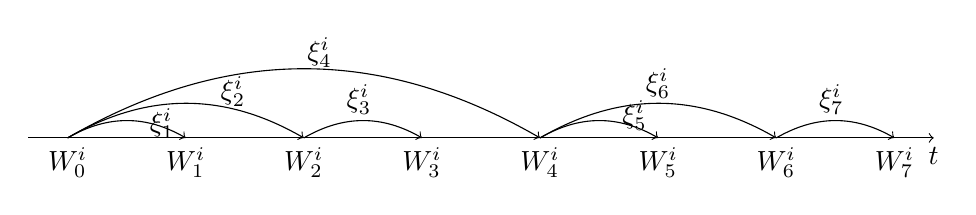
\begin{tikzpicture}
\path (0.5, 0) coordinate (A) node[below] {$W_0^i$};
\path (2, 0) coordinate (B) node[below] {$W_1^i$};
\path (3.5, 0) coordinate (C) node[below] {$W_2^i$};
\path (5, 0) coordinate (D) node[below] {$W_3^i$};
\path (6.5, 0) coordinate (E) node[below] {$W_4^i$};
\path (8, 0) coordinate (F) node[below] {$W_5^i$};
\path (9.5, 0) coordinate (G) node[below] {$W_6^i$};
\path (11, 0) coordinate (H) node[below] {$W_7^i$};
\path (11.5, 0) coordinate (I) node[below] {$t$};
\path (3.7, 1.4) node[below] {$\xi_4^i$};
\path (8, 1) node[below] {$\xi_6^i$};
\path (10.2, 0.8) node[below] {$\xi_7^i$};
\path (1.7, 0.5) node[below] {$\xi_1^i$};
\path (2.6, 0.9) node[below] {$\xi_2^i$};
\path (4.2, 0.8) node[below] {$\xi_3^i$};
\path (7.7, 0.6) node[below] {$\xi_5^i$};
\draw (0,0) edge[->] (11.5,0);
    \path[->] (A) edge [bend left] node [right] {} (B);
     \path[->] (A) edge [bend left] node [right] {} (C);
     \path[->] (C) edge [bend left] node [right] {} (D);
     \path[->] (A) edge [bend left] node [right] {} (E);
     \path[->] (E) edge [bend left] node [right] {} (F);
     \path[->] (E) edge [bend left] node [right] {} (G);
     \path[->] (G) edge [bend left] node [right] {} (H);
\end{tikzpicture}

\end{document}